\renewcommand{\FileName}{logit}
\begin{frame}
	\frametitle{Modeling approaches: Overview}
\begin{center}
\includegraphics[height=.83\textheight]{fig/assoc-resp-models}
\end{center}
\end{frame}

\begin{frame}<old>
\frametitle{Logit models}
For a \emph{binary} response, each \loglin\ model is equivalent to a logit
model (logistic regression, with categorical predictors)
  \begin{itemize}
	\item<1-> Admit $\perp$ Gender \given Dept (conditional independence $\equiv$ [AD][DG])
	\begin{equation*}
%	  [AD][GD] \equiv
	  \log \,  m_{ijk}  =
	  \mu
	  +  \lambda_i^A
	  +  \lambda_j^D
	  +  \lambda_k^G
	  +  \lambda_{ij}^{AD}
	  +  \lambda_{jk}^{DG}
	\end{equation*}
	\begin{equation*}
	\leftrightarrow L_{jk} = \log (m_{1jk} / m_{2jk}) 
	= (\lambda_1^A - \lambda_2^A) + (\lambda_{1j}^{AD} - \lambda_{2j}^{AD})
	=\alpha   +  \beta _j^{\mbox{\scriptsize Dept}} 
	\end{equation*}

	\item<2-> Admit $\perp$ Gender \given Dept, except for Dept. A
	\begin{equation*}
	  \log \,  m_{ijk}  =
	  \mu
	  +  \lambda_i^A
	  +  \lambda_j^D
	  +  \lambda_k^G
	  +  \lambda_{ij}^{AD}
	  +  \lambda_{jk}^{DG}
	  +  \delta_{(j=1)} \lambda_{ik}^{AG}
	\end{equation*}
	\begin{equation*}
	\leftrightarrow  L_{ij}  = \log (m_{1jk} / m_{2jk}) = 
	   \alpha   +  \beta _j^{\mbox{\scriptsize Dept}}
	   +  \delta_{(j=1)} \beta^{\mbox{\scriptsize Gender}}
	\end{equation*}
	   where,
	   \begin{itemize*}
	   \item $L_{ij} = \log (m_{ij1} / m_{ij2})$: log odds of
	   admission,
	   \item $\beta _j^{\mbox{\scriptsize Dept}}$: effect on admissions of department,
	   \item $\delta_{(j=1)} \beta^{\mbox{\scriptsize Gender}}$: 1 df term for effect of gender in Dept. A.
	   \item associations among predictors are \alert{assumed}, but don't appear in the logit model
	   \end{itemize*}
  \end{itemize} 
\end{frame}

\begin{frame}
\frametitle{Logit models}
For a \emph{binary} response, each \loglin\ model is equivalent to a logit
model (logistic regression, with categorical predictors)
  \begin{itemize}
	\item e.g., Admit $\perp$ Gender \given Dept (conditional independence $\equiv$ [AD][DG])
	\begin{equation*}
%	  [AD][GD] \equiv
	  \log \,  m_{ijk}  =
	  \mu
	  +  \lambda_i^A
	  +  \lambda_j^D
	  +  \lambda_k^G
	  +  \lambda_{ij}^{AD}
	  +  \lambda_{jk}^{DG}
	\end{equation*}
    So, for admitted ($i=1$) and rejected ($i=2$), we have:
	\begin{eqnarray}
	  \log m_{1jk}  = \cancel{\mu} +  \lambda_1^A +  \cancel{\lambda_j^D} +  \cancel{\lambda_k^G} +  \lambda_{1j}^{AD} +  \cancel{\lambda_{jk}^{DG}}  \label{eq:adm}\\
	  \log m_{2jk}  = \cancel{\mu} +  \lambda_2^A +  \cancel{\lambda_j^D} +  \cancel{\lambda_k^G} +  \lambda_{2j}^{AD} +  \cancel{\lambda_{jk}^{DG}}  \label{eq:rej}
	\end{eqnarray}

    Thus, subtracting \eqref{eq:adm}-\eqref{eq:rej}, terms not involving Admit will cancel:
	\begin{eqnarray*}
	L_{jk} & = & \log m_{1jk} - \log m_{2jk} = \log (m_{1jk} / m_{2jk}) = \mbox{\alert{log odds of admission}} \\
	       & = & (\lambda_1^A - \lambda_2^A) + (\lambda_{1j}^{AD} - \lambda_{2j}^{AD}) \\
		   & = & \alpha   +  \beta _j^{\mbox{\scriptsize Dept}} \quad\quad\quad\mbox{\alert{(renaming terms)}}
	\end{eqnarray*}
	 

	   where,
	   \begin{itemize*}
%	   \item $L_{jk} = \log (m_{1jk} / m_{2jk})$: log odds of admission,
       \item $\alpha$: overall log odds of admission
	   \item $\beta _j^{\mbox{\scriptsize Dept}}$: effect on admissions of department,
%	   \item $\delta_{(j=1)} \beta^{\mbox{\scriptsize Gender}}$: 1 df term for effect of gender in Dept. A.
	   \item associations among predictors are \alert{assumed}, but don't appear in the logit model
	   \end{itemize*}
%	  \end{itemize*}
  \end{itemize}
 \end{frame}

\begin{frame}
\frametitle{Logit models}
Other loglinear models have similar, simpler forms as logit models, where only the relations of
the response to the predictors appear in the equivalent logit model.
  \begin{itemize}
	\item<1-> Admit $\perp$ Gender $\perp$ Dept (mutual independence $\equiv$ [A][D][G])
	\begin{eqnarray*}
	  \log  m_{ijk}  & = & \mu +  \lambda_i^A +  \lambda_j^D  +  \lambda_k^G \\
	  \equiv L_{jk}  & = & (\lambda_1^A - \lambda_2^A) = \alpha \quad\quad\mbox{\alert{(constant log odds)}}
	\end{eqnarray*}

	\item<2-> Admit $\perp$ Gender \given Dept, except for Dept. A
	\begin{eqnarray*}
	  \log  m_{ijk} & = & \mu +  \lambda_i^A +  \lambda_j^D +  \lambda_k^G
	                    +  \lambda_{ij}^{AD} +  \lambda_{jk}^{DG} +  \delta_{(j=1)} \lambda_{ik}^{AG} \\
	  \equiv L_{jk}  & = &	\log (m_{1jk} / m_{2jk}) = 
	   \alpha   +  \beta _j^{\mbox{\scriptsize Dept}}
	   +  \delta_{(j=1)} \beta^{\mbox{\scriptsize Gender}}			
	\end{eqnarray*}


%\begin{comment}
%	\begin{equation*}
%	  \log \,  m_{ijk}  =
%	  \mu
%	  +  \lambda_i^A
%	  +  \lambda_j^D
%	  +  \lambda_k^G
%	  +  \lambda_{ij}^{AD}
%	  +  \lambda_{jk}^{DG}
%	  +  \delta_{(j=1)} \lambda_{ik}^{AG}
%	\end{equation*}
%	\begin{equation*}
%	\leftrightarrow  L_{ij}  = \log (m_{1jk} / m_{2jk}) = 
%	   \alpha   +  \beta _j^{\mbox{\scriptsize Dept}}
%	   +  \delta_{(j=1)} \beta^{\mbox{\scriptsize Gender}}
%	\end{equation*}
%\end{comment}

	   where,
	   \begin{itemize*}
%	   \item $L_{jk} = \log (m_{1jk} / m_{2jk})$: log odds of admission,
	   \item $\beta _j^{\mbox{\scriptsize Dept}}$: effect on admissions for department $j$,
	   \item $\delta_{(j=1)} \beta^{\mbox{\scriptsize Gender}}$: 1 df term for effect of gender in Dept. A.
%	   \item associations among predictors are \alert{assumed}, but don't appear in the logit model
	   \end{itemize*}
  \end{itemize} 
\end{frame}

\subsection{Fitting logit models}
\begin{frame}	
\frametitle{Logit models: Overview}
  \begin{itemize}
	\item{\large\bfseries Fitting procedures}
      \begin{itemize*}
	  \item \PROC{CATMOD}, \PROC{LOGISTIC} 
	  \item \PROC{GENMOD} \texttt{/ dist=poisson}
%	  \item \INSIGHT\ (Fit Y X) Options $\rightarrow$ Distribution poisson
	  \item SPSS: Logistic regression, Loglinear $\rightarrow$ Logit, Generalized Linear Models
	  \item R: glm(), gnm()
	  \end{itemize*}
	\item{\large\bfseries Visualization procedures}
      \begin{itemize*}
	  \item \macro{CATPLOT} - plot predicted, observed log odds from
	  \texttt{CATMOD}
	  \item \macro{INFLGLIM} - influence plots for generalized linear models
	  \item \macro{HALFNORM} - half-normal plot of residuals for generalized linear models
	  \end{itemize*}
	\item{\large\bfseries SAS craft}
      \begin{itemize*}
	  \item All SAS procedures $\rightarrow$ \ODS\ with obs., fitted values, residuals, diagnostics, etc.
	  \item New model $\rightarrow$ new \ODS\
	  \item Plotting steps remain the same
	  \item Similar ideas for SPSS, R
	  \end{itemize*}
  \end{itemize}

\end{frame}


\subsection{Plots for logit models}
\begin{frame}[fragile]
%\makeatletter\slidebox@restore\makeatother
\frametitle{Plots for logit models}
\begin{itemize}
\item Fit: \PROC{CATMOD}; plot: \macro{CATPLOT}
\item Model: Admit $\sim$ Gender + Dept $\leftrightarrow$ \loglin\ [AD] [AG] [DG]
\begin{listing}[frame=single,baselinestretch=0.8]
proc catmod order=data data=berkeley;
   weight freq;
   response / \sasemph{out=predict};
   model \sasemph{admit = dept gender} / ml;
%catplot(\sasemph{data=predict}, xc=dept, class=gender,
    type=FUNCTION, z=1.96, legend=legend1);
\end{listing}

\begin{center}
  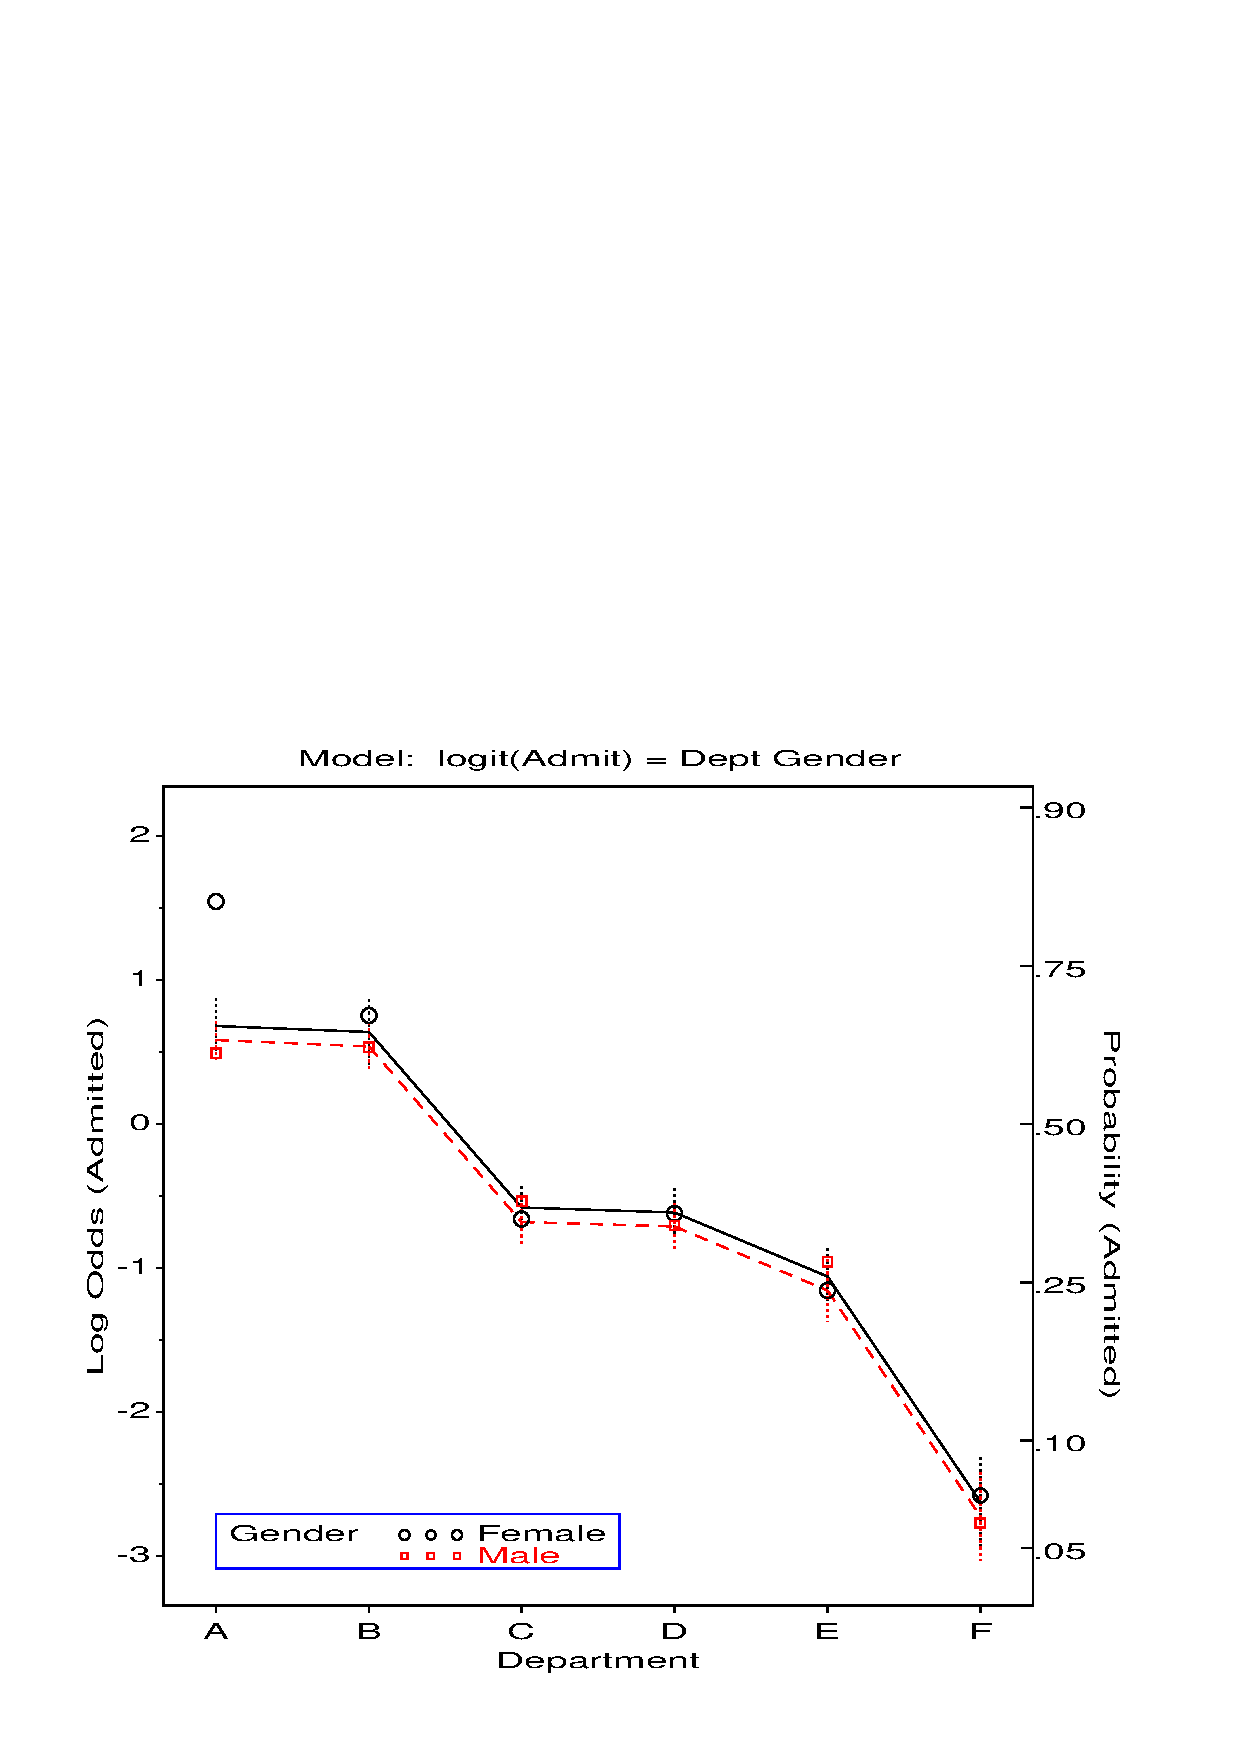
\includegraphics[width=.43\dispwidth,clip]{fig/catberk2}
\end{center}
\end{itemize}
\end{frame}

\begin{frame}
\frametitle{Plots for logit models}
 \begin{columns}
  \begin{column}{.5\textwidth}
     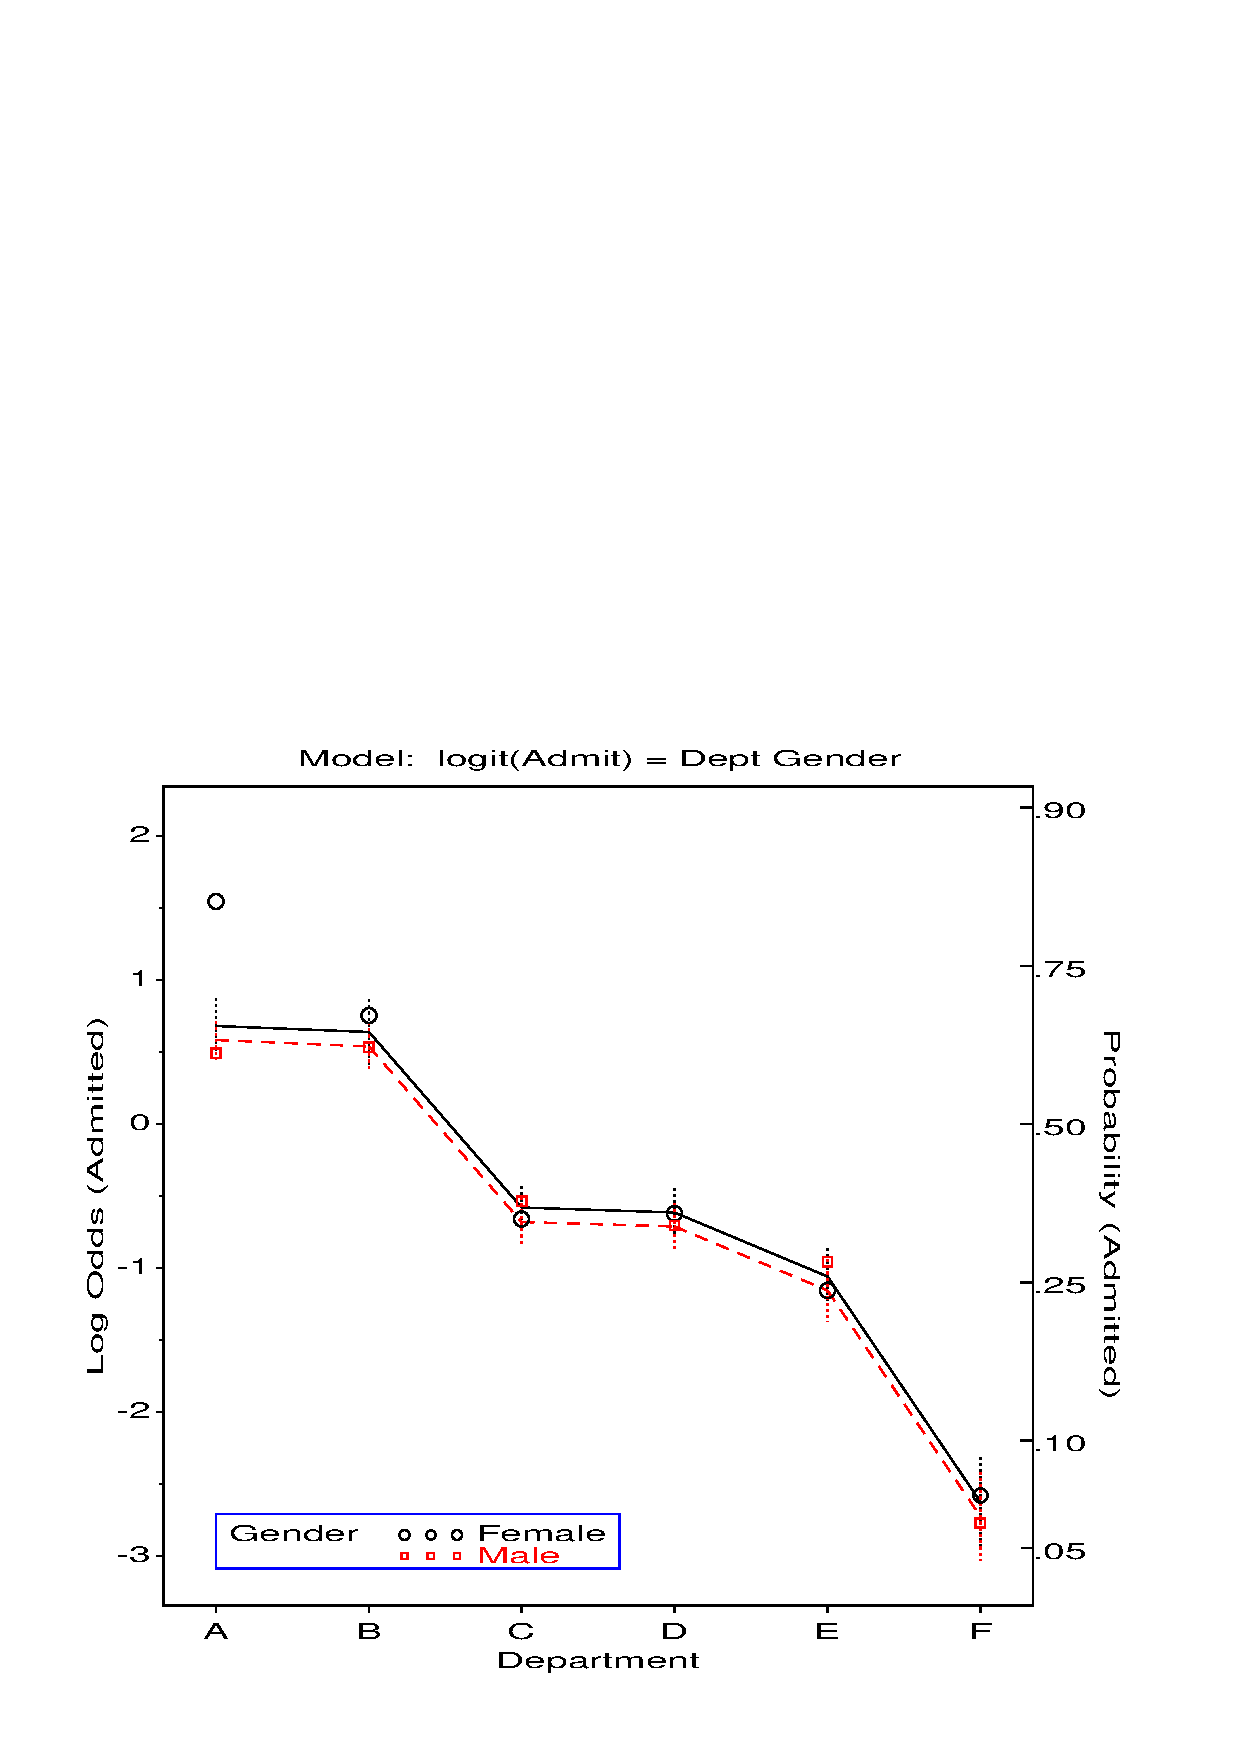
\includegraphics[width=\linewidth,clip]{fig/catberk2}
  \end{column}
  \begin{column}{.5\textwidth}
     \begin{itemize}
      \item Plots \alert{observed} and \alert{predicted} on the logit scale (type=FUNCTION)
      \item[$\Rightarrow$] Main effects model--- parallel profiles
      \item Probabilities on a separate scale (added below)
     \end{itemize}
  \end{column}
 \end{columns}
 
\end{frame}

\begin{frame}[fragile]
  \frametitle{Logit models: details}
  \begin{itemize}
	\item{\large\bfseries Model:} Admit $\sim$ Gender + Dept $\leftrightarrow$ [AD] [AG] [DG]
  \end{itemize}
\vspace{2ex}
\begin{Input}[fontsize=\small,label=\fbox{\texttt{catberk2.sas} $\cdots$},baselinestretch=0.7]
%include catdata(berkeley);
proc catmod order=data
            data=berkeley;
   weight freq;
   response / out=predict;
   model admit = dept gender / ml;
  run;
\end{Input}
\PROC{CATMOD} output:  Overall tests and goodness of fit
\begin{Output}[gobble=7,baselinestretch=0.7]
                    Maximum Likelihood Analysis of Variance
 
               Source               DF   Chi-Square    Pr > ChiSq
               --------------------------------------------------
               Intercept             1       262.49        <.0001
               dept                  5       534.78        <.0001
               gender                1         1.53        0.2167

               \sasemph{Likelihood Ratio      5        20.20        0.0011}
\end{Output}
\begin{itemize*}
  \item No effect of Gender; big effect of Dept 
  \item LR test (vs. saturated model): Model doesn't fit well---  Why? How to  modify?
\end{itemize*}
\end{frame}

\begin{frame}[fragile]
  \frametitle{Plots for logit models: Output data set}
\PROC{CATMOD} output data set: observed \& predicted, probabilities \& logits
\begin{Output}[gobble=0,baselinestretch=0.7,fontsize=\footnotesize]
dept    gender    admit     _TYPE_       _OBS_    _PRED_    _SEPRED_

 A      Male                FUNCTION     0.492     0.582      0.069 
 A      Male      Admit     PROB         0.621     0.642      0.016 
 A      Male      Reject    PROB         0.379     0.358      0.016 
 A      Female              FUNCTION     1.544     0.682      0.099 
 A      Female    Admit     PROB         0.824     0.664      0.022 
 A      Female    Reject    PROB         0.176     0.336      0.022 
 B      Male                FUNCTION     0.534     0.539      0.086 
 B      Male      Admit     PROB         0.630     0.631      0.020 
 B      Male      Reject    PROB         0.370     0.369      0.020 
 B      Female              FUNCTION     0.754     0.639      0.116 
 B      Female    Admit     PROB         0.680     0.654      0.026 
 B      Female    Reject    PROB         0.320     0.346      0.026
 ...
 F      Male                FUNCTION    -2.770    -2.724      0.158 
 F      Male      Admit     PROB         0.059     0.062      0.009 
 F      Male      Reject    PROB         0.941     0.938      0.009 
 F      Female              FUNCTION    -2.581    -2.625      0.158 
 F      Female    Admit     PROB         0.070     0.068      0.010 
 F      Female    Reject    PROB         0.930     0.932      0.010 
\end{Output}
This contains both the observed and fitted logit values (\verb|_TYPE_='FUNCTION'|)
and probabilities (\verb|_TYPE_='PROB'|)
\end{frame}

\begin{frame}[fragile]
\frametitle{\macrot{CATPLOT}}
\begin{itemize*}
  \item Plot logit values (\verb|_TYPE_='FUNCTION'|) or probabilities
  (\verb|_TYPE_='PROB'|)
  \item With \macro{PSCALE}, can plot on logit scale, with probability scale on
  right.
\end{itemize*}
\vspace{2ex}
\begin{Input}[fontsize=\small,label=\fbox{$\cdots$ \texttt{catberk2.sas}},baselinestretch=0.8,firstnumber=9]

\sasemph{%pscale(lo=-4, hi=3, anno=pscale);}

title 'Model:  logit(Admit) = Dept Gender'
   a=-90 'Probability (Admitted)';
axis1 order=(-3 to 2) offset=(4)
      label=(a=90 'Log Odds (Admitted)');
axis2 label=('Department') offset=(4);
%catplot(data=predict, class=gender, xc=dept,
    \sasemph{type=FUNCTION},     \sascomment{/* plot logit values         */}
    z=1.96,            \sascomment{/* show 1.96 x SE -> 95\% CI */}
    \sasemph{anno=pscale});      \sascomment{/* add probability scale     */}
\end{Input}
\end{frame}

\subsection{CATPLOT macro}
\begin{frame}
\frametitle{\macrot{CATPLOT}}
\begin{center}
  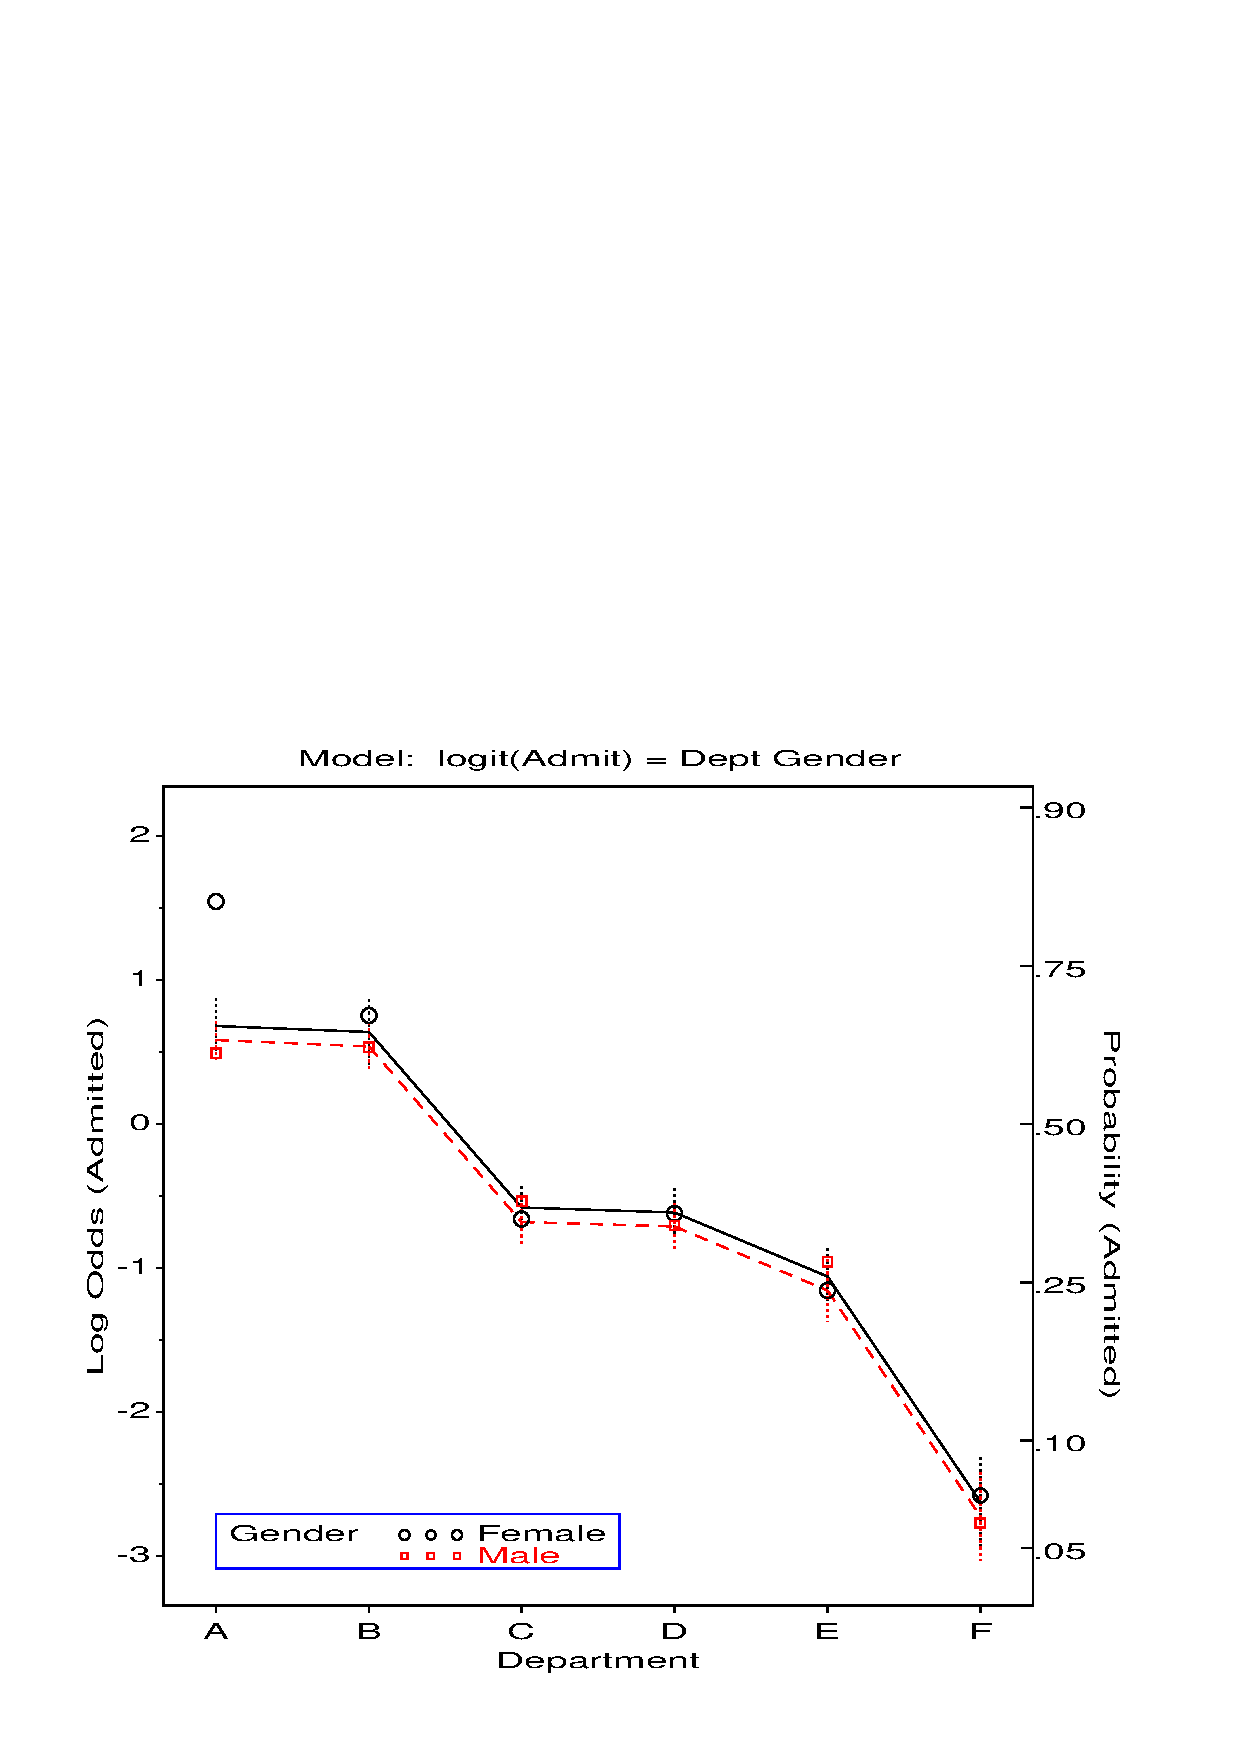
\includegraphics[height=.8\textheight,clip]{fig/catberk2}
\end{center}
$\rightarrow$ no effect of Gender, except in Dept A (Females more likely admitted!)
\end{frame}

\begin{frame}[fragile]
  \frametitle{Fitting and graphing other models}
  \begin{itemize*}
  \item Change \texttt{MODEL} statement $\rightarrow$ new fitted values
  \item Plotting step remains the same
  \item Admit $\perp$ Gender \given Dept, except for Dept. A $\leftrightarrow$ Admit $\sim$  Dept + $\delta_{j=1}$ Gender
\begin{listing}
proc catmod order=data data=berkeley;
   response / out=predict;
   model \sasemph{admit = dept dept1AG} / ml;
%catplot(data=predict, xc=dept, class=gender,
    type=FUNCTION, z=1.96, legend=legend1);
\end{listing}

  \begin{center}
	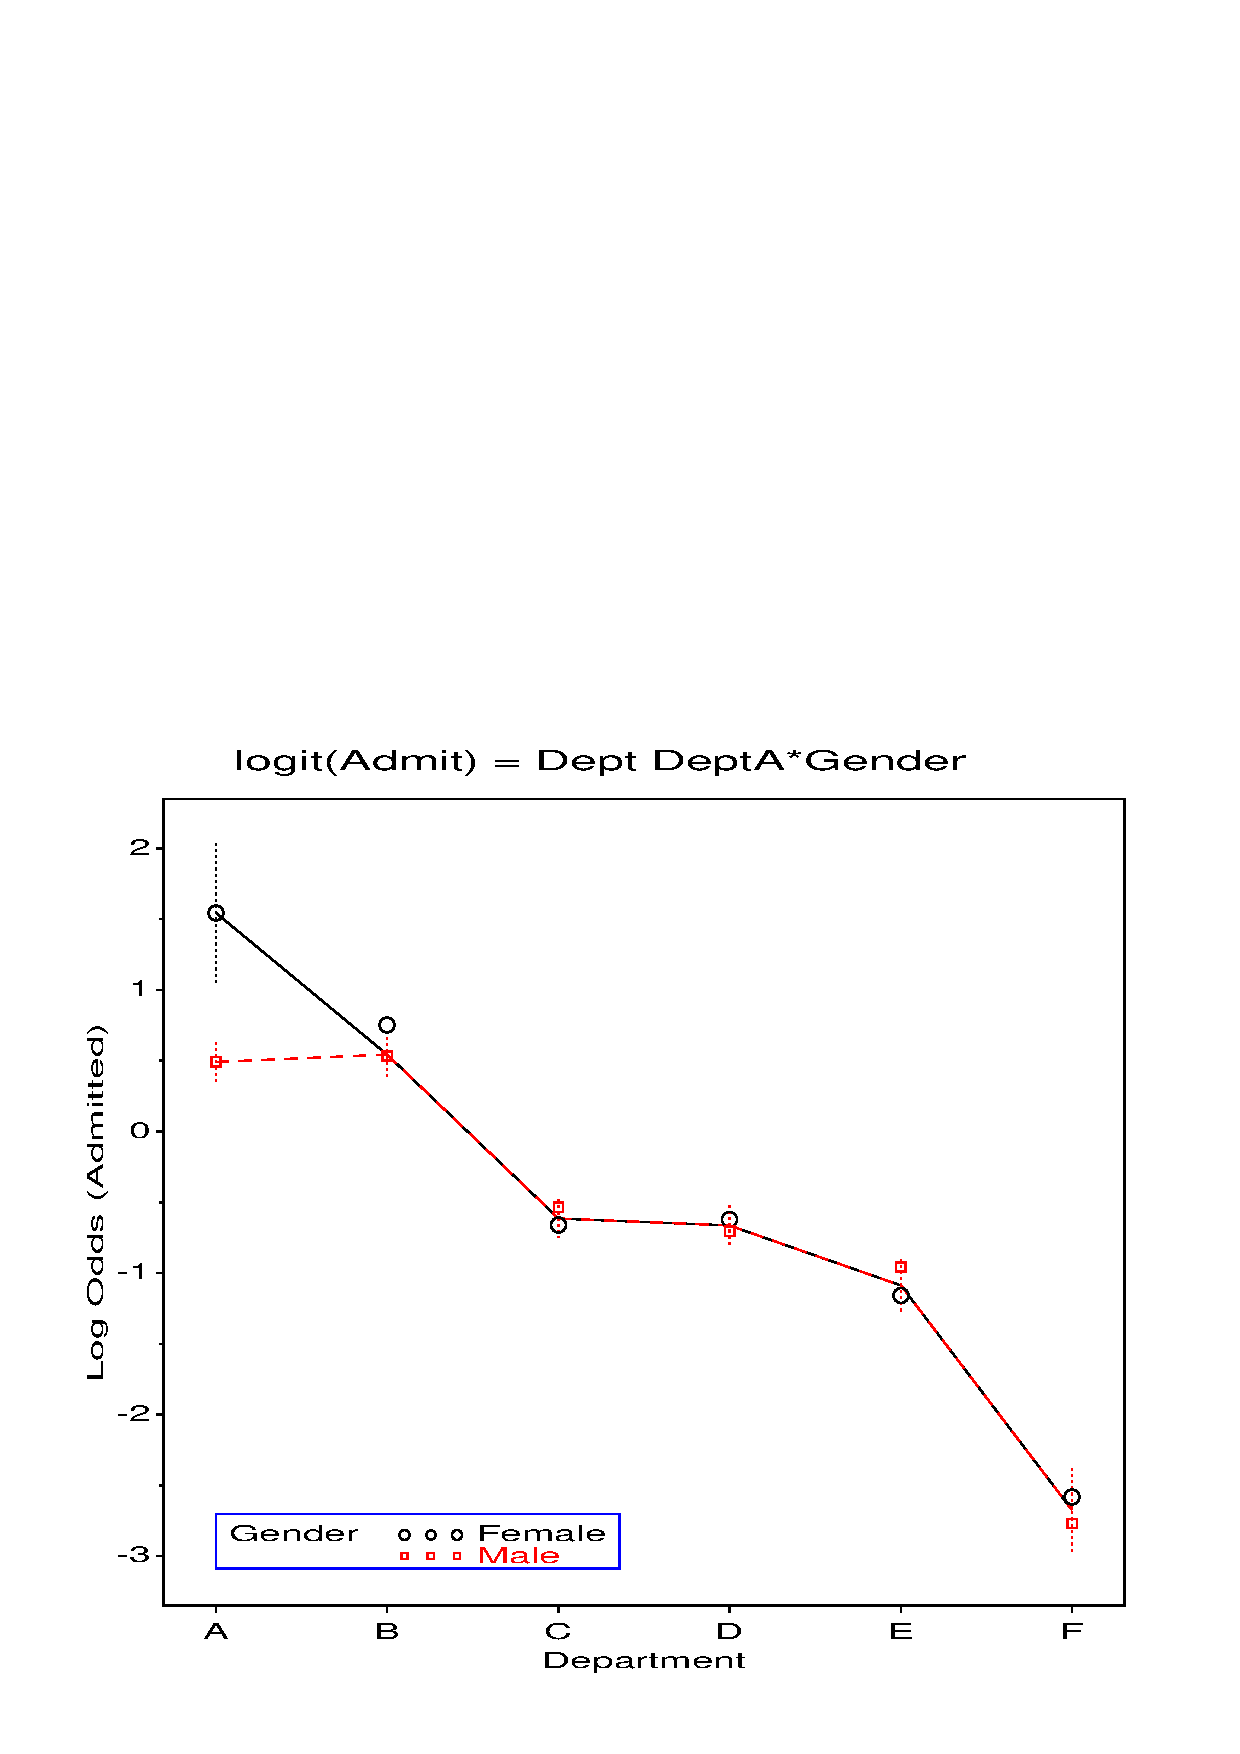
\includegraphics[width=.4\dispwidth,clip]{fig/catberk6}
  \end{center}
  \end{itemize*}
\end{frame}

\begin{frame}[fragile]
  \frametitle{Fitting and graphing other models: details}
  \begin{itemize}
  \item Model: Admit $\perp$ Gender \given Dept, except for Dept. A
  \item Need to define a dummy variable for effect of Gender in Dept. A 
  \end{itemize}
  \vspace{1ex}
\begin{Input}[fontsize=\small,label=\fbox{\texttt{catberk6.sas} $\cdots$},baselinestretch=0.75]
%include catdata(berkeley);
data berkeley;
   set berkeley;
   \sascomment{*-- Dummy variable for Gender in Dept A;}
   \sasemph{dept1AG = (gender='F') *  (dept=1);}
   format dept dept.;

proc catmod order=data
            data=berkeley;
   weight freq;
   population dept gender;
   direct dept1AG;
   response / out=predict;
   model \sasemph{admit = dept dept1AG} / ml;
  run;
  ...
\end{Input}
\end{frame}

\begin{frame}[fragile]
   \frametitle{Fitting and graphing other models:details}
\PROC{CATMOD} output:
\begin{Output}[baselinestretch=0.7]
          Maximum Likelihood Analysis of Variance

     Source               DF   Chi-Square    Pr > ChiSq
     --------------------------------------------------
     Intercept             1       291.22        <.0001
     dept                  5       571.45        <.0001
     dept1AG               1        16.04        <.0001

     \sasemph{Likelihood Ratio      5         2.68        0.7489}

          Analysis of Maximum Likelihood Estimates

                          Standard      Chi-
Parameter      Estimate      Error    Square  Pr > ChiSq
--------------------------------------------------------
Intercept       -0.6685     0.0392    291.22      <.0001
dept      A      1.1606     0.0705    271.21      <.0001
          B      1.2113     0.0802    227.95      <.0001
          C      0.0528     0.0687      0.59      0.4426
          D     0.00358     0.0727      0.00      0.9607
          E     -0.4210     0.0871     23.34      <.0001
dept1AG          1.0521     0.2627     16.04      <.0001
\end{Output}
Fits well! How to interpret?
\end{frame}

\begin{frame}[fragile]
   \frametitle{Fitting and graphing other models: details}
\PROC{CATMOD}: observed and predicted logits:
\vspace{1ex}
\begin{Input}[label=\fbox{$\cdots$ \texttt{catberk6.sas} $\cdots$},firstnumber=17]
proc print data=predict;
  id dept gender;
  var _obs_ _pred_ _sepred_;
  format _numeric_  6.3 dept dept.;
  \sasemph{where(_type_='FUNCTION');}
\end{Input}
\begin{Output}[baselinestretch=0.7,gobble=6]
           dept    gender     _OBS_    _PRED_    _SEPRED_

            A        M        0.492     0.492      0.072 
            A        F        1.544     1.544      0.253 
            B        M        0.534     0.543      0.086 
            B        F        0.754     0.543      0.086 
            C        M       -0.536    -0.616      0.069 
            C        F       -0.660    -0.616      0.069 
            D        M       -0.704    -0.665      0.075 
            D        F       -0.622    -0.665      0.075 
            E        M       -0.957    -1.090      0.095 
            E        F       -1.157    -1.090      0.095 
            F        M       -2.770    -2.676      0.152 
            F        F       -2.581    -2.676      0.152 
\end{Output}

\end{frame}

\begin{frame}[fragile]
   \frametitle{Fitting and graphing other models: details}
\vspace{1ex}
\begin{Input}[label=\fbox{$\cdots$ \texttt{catberk6.sas}},firstnumber=22]
title 'logit(Admit) = Dept DeptA*Gender';
%catplot(data=predict, x=dept, class=gender, 
   type=FUNCTION,      \sascomment{/* plot the log odds */}
   z=1.96);            \sascomment{/* 95\% error bars    */}
\end{Input}
\begin{center}
  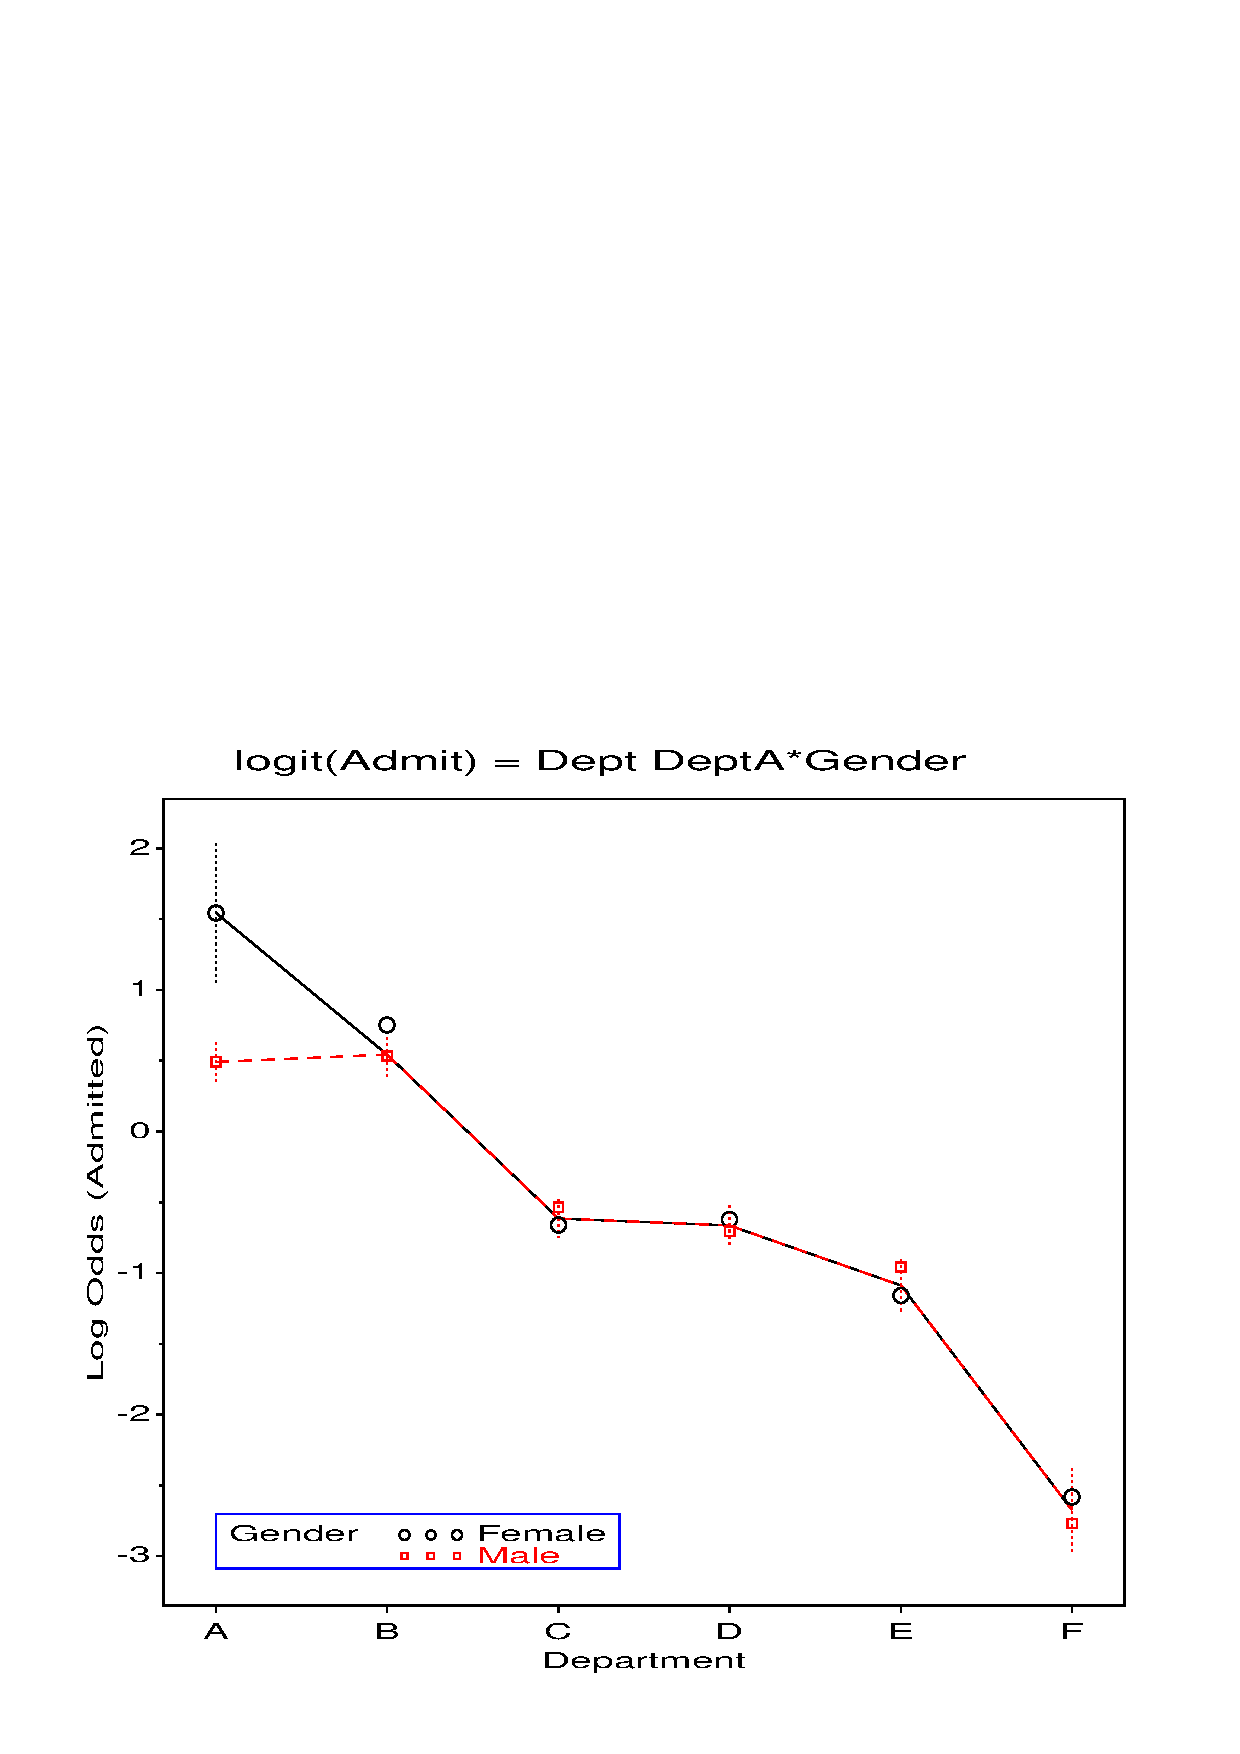
\includegraphics[width=.55\dispwidth,clip]{fig/catberk6}
\end{center}

\end{frame}


\subsection{Diagnostic plots for GLMs}
\begin{frame}
%\iflandscape\def\dispfactor{.4}\else \def\dispfactor{.8}\fi
\frametitle{Diagnostic plots for Generalized Linear Models}
\macro{INFLGLIM}: Influence plots for generalized linear models \citep{Williams:87}
  \begin{itemize*}
  \item Fit: \PROC{GENMOD}; calculates additional diagnostic measures
  (Hat value, Cook's D, etc.)
  \item Plot: measures of residual (\texttt{GY}=$\Delta \chi^2$, $\chi^2$ residual) vs.
  leverage (\texttt{GX}=hat value),  bubble size (area, radius) $\sim$ Cook's D.
  \item $\rightarrow$ which cells have undue impact on fitted model?
  \end{itemize*}
\begin{center}
  \includegraphics[width=.4\dispwidth,clip]{fig/genberk1}
\end{center}

\end{frame}

\begin{frame}[fragile]
\frametitle{\macrot{INFLGLIM}: Example}
\begin{itemize*}
  \item Berkeley data, model $[AD][GD] \leftrightarrow L_{ij}   = 
	\alpha   +  \beta _j^{\mbox{\scriptsize Dept}} $
  \vspace{3ex}
\begin{Input}[label=\fbox{\texttt{genberk1.sas}}]
%include catdata(berkeley);
\sascomment{*-- make a cell ID variable, joining factors;}
data berkeley;
   set berkeley;
   cell = trim(put(dept,dept.)) ||
          gender ||
          trim(put(admit,yn.));
 
%inflglim(data=berkeley, 
   class=dept gender admit,
   resp=freq, 
   model=admit|dept gender|dept, 
   dist=poisson, 
   id=cell,
   \sasemph{gx=hat, gy=streschi});
\end{Input}
\end{itemize*}

\end{frame}

\begin{frame}
\frametitle{\macrot{INFLGLIM}: Example}
\begin{center}
  \includegraphics[width=.6\dispwidth,clip]{fig/genberk1}
\end{center}
\begin{itemize*}

\item All cells which do not fit ($|r_i| > 2$) are for department A.
\item Males applying to dept A 
have large leverage $\Rightarrow$  large influence (Cook's D)
\end{itemize*}
\end{frame}

\begin{frame}[fragile]
\frametitle{Influence plots in R}
The \func{influencePlot} function in the \pkg{car} gives similar plots:
\vspace{1.2ex}
\begin{Input}[label=\fbox{\texttt{berkeley-diag.R}},baselinestretch=0.8]
berkeley <- as.data.frame(UCBAdmissions)
 ...
berk.mod <- glm(Freq ~ Dept * (Gender+Admit), data=berkeley, 
                family="poisson")
influencePlot(berk.mod, id.n=3, id.col="red")
\end{Input}
% $ end math mode in editor
\begin{center}
\includegraphics[width=.45\dispwidth,clip]{fig/berkeley-diag}
\end{center}
\end{frame}

\begin{frame}[fragile]
\frametitle{Diagnostic plots for Generalized Linear Models}
\macro{HALFNORM}: Half-normal plot of residuals \citep{Atkinson:81}
   \begin{itemize*}
   \item Plot ordered \emph{absolute} residuals, $| r |_{(i)}$ vs. expected normal values, $| z |_{(i)}$
   \item Standard normal confidence envelope not suitable for GLMs
   \item Simulate reference `line' and envelope with simulated confidence intervals 
   \end{itemize*}

\vspace{2ex}
\begin{Input}[label=\fbox{$\cdots$ \texttt{genberk1.sas}}]
%halfnorm(data=berkeley, 
   class=dept gender admit,
   resp=freq, 
   model=dept|gender dept|admit, 
   dist=poisson, id=cell);
\end{Input}
\end{frame}

\begin{frame}
\begin{center}
  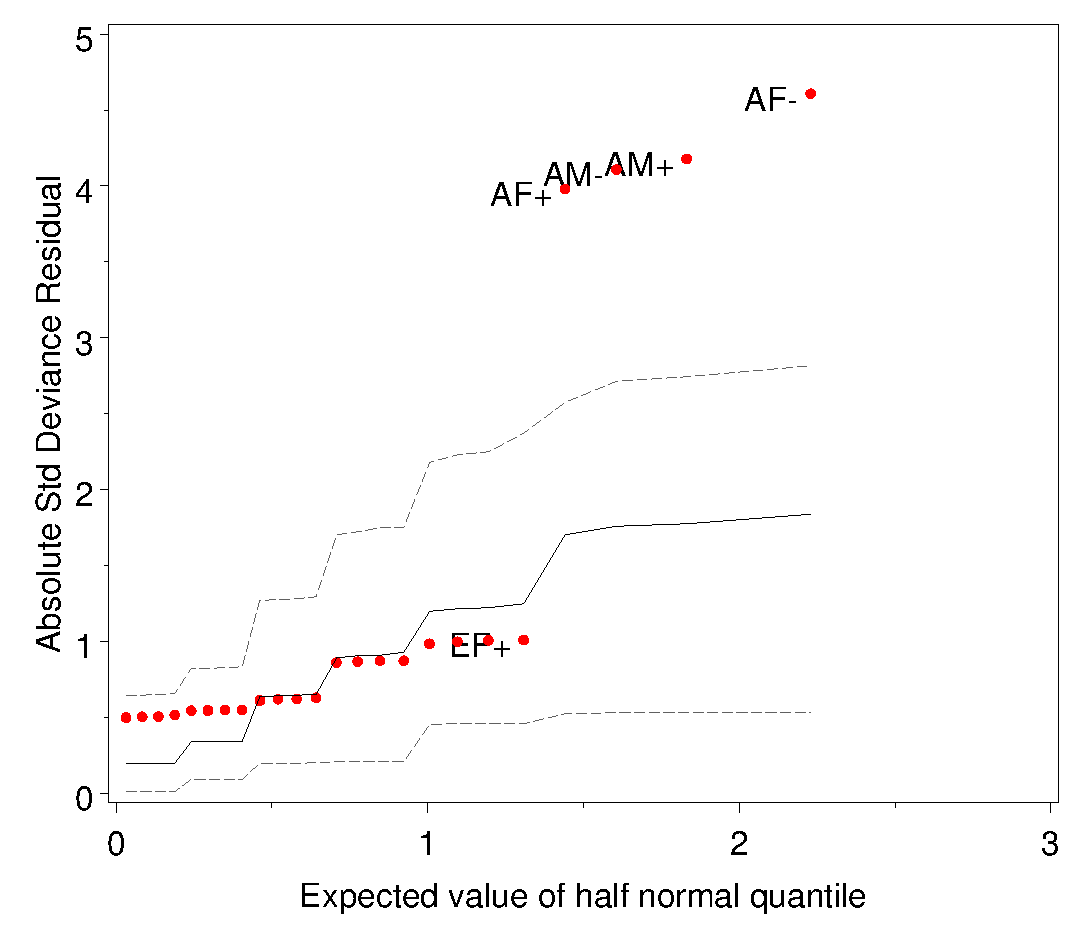
\includegraphics[width=.7\dispwidth,clip]{fig/genberk13}
\end{center}
\begin{itemize*}
\item Points with largest $|$residual$|$ labeled
\item The model fits well, except in department A.
%\item Strong evidence for \emph{lack} of gender bias, controlling for department 
%\item (possibility of structural bias not tested)
\end{itemize*}

\end{frame}

\endinput
% slide template
\begin{frame}
  \frametitle{}
  \begin{itemize}
	\item{\large\bfseries }
      \begin{itemize*}
	  \item 
    	\begin{itemize*}
		\item 
		\item 
		\end{itemize*}
	  \item 
	  \end{itemize*}
	\item{\large\bfseries }
	\item{\large\bfseries }
  \end{itemize}
\end{frame}

